\subsection{Composite}

\begin{figure}[htb]
	\caption{\label{fig_grafico}Estrutura do Composite}
	\begin{center}
	    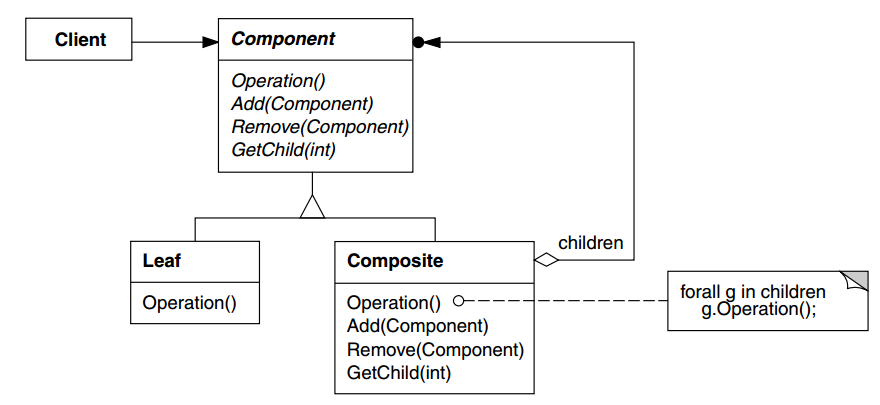
\includegraphics[scale=0.5]{5_padroes-contexto-funcional/5.2_estruturais/5.2.3_composite/diagram.png}
	\end{center}
\end{figure}

Exemplo Orientado a Objetos:

\begin{lstlisting}[caption={Composite Orientado a Objetos},label=oocomposite]



\end{lstlisting}

Contexto Funcional:


\begin{lstlisting}[caption={Composite Funcional},label=fpcomposite]
    

    
\end{lstlisting}